%% Manuscript for Springer journal 41062 (Springer Nature LaTeX template, sn-jnl, Basic reference style).
%% Numbers quoted in the text are macros from generated/numbers.tex (scripts/paper_tables.py); tables are
%% \input from generated/. Regenerate both after any rerun instead of editing numbers by hand.

\documentclass[pdflatex,sn-basic]{sn-jnl}

\usepackage{graphicx}
\usepackage{multirow}
\usepackage{amsmath,amssymb,amsfonts}
\usepackage{xcolor}
\usepackage{textcomp}
\usepackage{booktabs}
\usepackage{siunitx}
\usepackage[title]{appendix}

\input{generated/numbers.tex}
\input{generated/series_numbers.tex}

\raggedbottom

\begin{document}

\title[Synthetic data augmentation for small structural datasets]{Does synthetic data augmentation improve
strength prediction for small structural test databases? A benchmark of five tabular generators with a
pre-registered training-size experiment}

\author[1]{\fnm{Danish} \sur{Dubey}}\email{danish.dubey.civ23@itbhu.ac.in}
\author[2]{\fnm{Ishan} \sur{Jha}}
\author*[1]{\fnm{Janhavi} \sur{Singh}}\email{janhavisingh.rs.civ22@itbhu.ac.in}
\author[1]{\fnm{Krishna Kant} \sur{Pathak}}

\affil[1]{\orgdiv{Department of Civil Engineering}, \orgname{Indian Institute of Technology (BHU) Varanasi},
\orgaddress{\city{Varanasi}, \postcode{221005}, \state{Uttar Pradesh}, \country{India}}}
\affil[2]{\orgname{Indian Institute of Technology (ISM) Dhanbad}, \orgaddress{\city{Dhanbad},
\state{Jharkhand}, \country{India}}}

\abstract{Experimental databases of composite structural members are small, and synthetic tabular data is
increasingly proposed as a way to enlarge them for machine-learning models. This study tests whether such
augmentation improves strength prediction when it is evaluated against a real-data baseline on identical test
data. Five generators (sequential CART, Gaussian Copula, CTGAN, CopulaGAN and TVAE) were benchmarked on 56 cyclic
tests of recycled aggregate concrete-filled steel tubular (RACFST) columns, with fold-local imputation and
generation inside repeated cross-validation and physical bounds enforced on every synthetic row. Sequential CART
reproduced the covariance structure of the data best. With 1:1 augmentation, the mean error of Random Forest and
XGBoost models for the ultimate lateral load was lower than that of models trained on the real data alone in
\regBetterOne{} of \regSettings{} settings, by at most \regBetterOnePctMax\%, and in none of these did the augmented
model win more than \regBetterOneWinsMax{} of 15 folds; an 11:1 synthetic-to-real ratio increased error in every
setting. A pre-registered experiment then varied the real
training size from 25 to 400 tests on 832 FRP-confined concrete specimens and 255 high-strength-steel rectangular
CFST columns. Across \eoneCells{} generator, regressor and size combinations, augmentation produced no
statistically supported benefit; it produced a statistically supported increase in error in \eoneHarm{}. The
results indicate that synthetic augmentation should not be assumed to help small structural datasets and that
any claimed benefit should be shown against a real-only baseline on the same test data.}

\keywords{Synthetic data, Data augmentation, Concrete-filled steel tube, FRP-confined concrete, Machine learning,
Pre-registration}

\maketitle

%% ---------------------------------------------------------------------------------------------------------
\section{Introduction}\label{sec:intro}

Machine-learning (ML) models are now widely used to predict the capacity of structural members from test
databases \citep{thai2022review}. For composite members such as concrete-filled steel tubular (CFST) columns and
fibre-reinforced polymer (FRP) confined concrete, these databases are compiled from many independent laboratory
programmes and remain small: a few dozen tests for specialised configurations such as recycled aggregate concrete
under cyclic loading \citep{xu2020racfst}, and a few hundred to a few thousand tests for the most studied member
types \citep{thai2019cfst,ozbakkaloglu2013database}. Small databases make ML predictions sensitive to which tests
fall in the training set and limit how far a model can be trusted outside the range of the data.

Synthetic tabular data has been proposed as a remedy. Generators fitted to the real tests produce additional
rows, which are added to the training set of the predictive model. Several families of generators are available
in open-source software: sequential classification and regression trees (CART), originally developed for
statistical disclosure control \citep{reiter2005cart,nowok2016synthpop}; copula models \citep{patki2016sdv}; and
deep generative models such as CTGAN, CopulaGAN and TVAE \citep{xu2019ctgan}. In structural engineering,
\citet{song2024fire} combined CTGAN with random oversampling to augment a database of CFST columns under fire and
reported improved prediction of fire resistance.

Whether augmentation helps depends on how it is evaluated. Synthetic rows are derived from the same training data
that the predictive model already sees, so they cannot add information about the physical system; any benefit
must come from a regularising effect on the learner. Detecting such an effect requires that (i) imputation and
generation are fitted only on the training portion of each split, so that no information from the test data
reaches the synthetic rows, (ii) the augmented model is compared with a model trained on the real training data
alone, evaluated on the same test data, and (iii) the comparison is repeated over enough splits for the
difference to be distinguished from split-to-split variation. The train-synthetic, test-real principle
\citep{esteban2017tstr} addresses the first requirement but not the other two.

This paper reports a benchmark designed to meet all three requirements. Its contributions are as follows.
\begin{enumerate}
\item Five generators from three families are compared on a database of 56 cyclic tests of recycled aggregate
concrete-filled steel tubular (RACFST) columns \citep{xu2020racfst}, with three missing-data treatments, physical
bounds enforced on every synthetic row, and imputation and generation repeated inside every cross-validation
fold. Fidelity, originality and predictive utility are reported for each generator.
\item The effect of the amount of synthetic data is measured by comparing 1:1 and approximately 11:1
synthetic-to-real ratios against a real-only baseline on identical folds.
\item A training-size experiment, with its design and decision rule registered in a public repository before it
was run \citep{nosek2018prereg}, tests whether augmentation helps when few real tests are available, on two
larger databases: FRP-confined concrete \citep{ozbakkaloglu2013database} and high-strength-steel rectangular CFST
columns \citep{thai2021reliability}.
\item The code, derived datasets and registration record are publicly available.
\end{enumerate}
An earlier version of the RACFST analysis was presented as an abstract at ICSRI-2026 \citep{dubey2026icsri}. The
present paper replaces its preliminary results with the corrected and extended analysis described below.

%% ---------------------------------------------------------------------------------------------------------
\section{Databases}\label{sec:data}

Four databases were used (Table~\ref{tab:data}). The RACFST database is the subject of the full benchmark
(Sect.~\ref{sec:e0}); the other three are used in the training-size experiment (Sect.~\ref{sec:e1}).

\begin{table}[t]
\caption{Databases used in this study}\label{tab:data}
\footnotesize
\setlength{\tabcolsep}{3pt}
\begin{tabular*}{\textwidth}{@{\extracolsep\fill}lllrll@{}}
\toprule
Database & Source & Target & Tests & Inputs & Use \\
\midrule
RACFST, cyclic & \citet{xu2020racfst}, App.\ A3 & $P_u$ (kN) & 56 & 13 + 3 derived & E0 \\
FRP-confined concrete & \citet{ozbakkaloglu2013database} & $f'_{cc}$ (MPa) & 832 & 13 & E1, registered \\
Rectangular HSS CFST & \citet{thai2021reliability} & $N$ (kN) & 255 & 9 & E1, registered \\
Circular HSS CFST & \citet{thai2021reliability} & $N$ (kN) & 93 & 8 & E1, exploratory \\
\bottomrule
\end{tabular*}
\end{table}

\subsection{RACFST columns under cyclic lateral loading}
\citet{xu2020racfst} compiled tests of recycled aggregate concrete-filled steel tubes under several loading
conditions. The 56 cyclic lateral-loading tests in their Appendix~A3 were used. Each test is described by section
shape (35 circular, 21 square), outer dimension $D$ (or $B$), wall thickness $t$, column length $2L$, recycled
coarse aggregate replacement ratio $r$, mix proportions (cement, sand, natural and recycled coarse aggregate,
water), concrete cube strength $f_{cu}$, steel yield strength $f_y$ and axial load ratio $n$. The mix proportions
are missing for 11 tests. The recycled fine aggregate content is zero for every test and is not used. The prediction target is the ultimate lateral load $P_u$ (39.1--195.5~kN).
The database also reports the displacement ductility coefficient $\mu$ and the equivalent viscous damping
coefficient $\xi$; these are measured outcomes of the same tests and are therefore not used as inputs. The
derived ratios $w/c$, $D/t$ and $L/D$ (with $L$ half the reported length $2L$) are removed before imputation and
generation and recomputed afterwards from their components, so that synthetic rows satisfy these identities
exactly. The $L/D$ values printed in the source table follow this definition for some studies and $2L/D$ for
others, and one specimen matches neither; the recomputed values use the same definition for every test.

\subsection{FRP-confined concrete}
\citet{ozbakkaloglu2013database} compiled 832 monotonic axial compression tests on circular FRP-confined concrete
specimens from 99 studies. The tables of the accepted manuscript were extracted to a machine-readable file with a
position-based parser. The extraction reproduces the stated total of 832 tests and the stated count of 77
tube-confined specimens, and the strain-reduction identity $k_\varepsilon = \varepsilon_{h,rup} /
\varepsilon_{frp}$ holds within 5\% for every row where both quantities are reported, except two rows whose
printed values are themselves inconsistent. The inputs are confinement type (CFRP, GFRP, AFRP, high-modulus CFRP,
or unbonded wrap or tube), specimen diameter and height, unconfined strength $f'_{co}$ and strain
$\varepsilon_{co}$, FRP composite and dry-fibre modulus, strength and thickness, ultimate axial strain
$\varepsilon_{cu}$ and hoop rupture strain $\varepsilon_{h,rup}$. The target is the confined strength $f'_{cc}$.
Between 20\% and 60\% of the values in the material-property and strain columns are missing, because studies
report either composite or fibre properties and not all report strains. $\varepsilon_{cu}$ and
$\varepsilon_{h,rup}$ are measured at failure; their use as inputs is discussed in Sect.~\ref{sec:limits}.

\subsection{High-strength-steel CFST columns}
The CFST database of \citet{thai2021reliability} (3,208 tests; published under CC BY 4.0
\citep{thai2021data}) was filtered to concentrically loaded columns with steel yield strength $f_y \geq
460$~MPa, the upper limit of the steel grades covered by Eurocode~4. This gives 255 rectangular and 93 circular
columns. The inputs are section dimensions, wall thickness, length, $f_y$, steel ultimate strength $f_u$, steel
modulus $E_a$, concrete strength $f_c$ and whether $f_c$ is a cylinder or cube value. $f_u$ and $E_a$ are missing
for about 40\% of rectangular and 50--67\% of circular columns. The target is the measured axial capacity $N$. The
circular subset was added after the training-size experiment had been registered and is reported as exploratory.

%% ---------------------------------------------------------------------------------------------------------
\section{Methods}\label{sec:methods}

The workflow for the RACFST benchmark is shown in Fig.~\ref{fig:flow}. The same components (imputation,
constrained generation, regressors) are reused in the training-size experiment.

\begin{figure}[t]
\centering
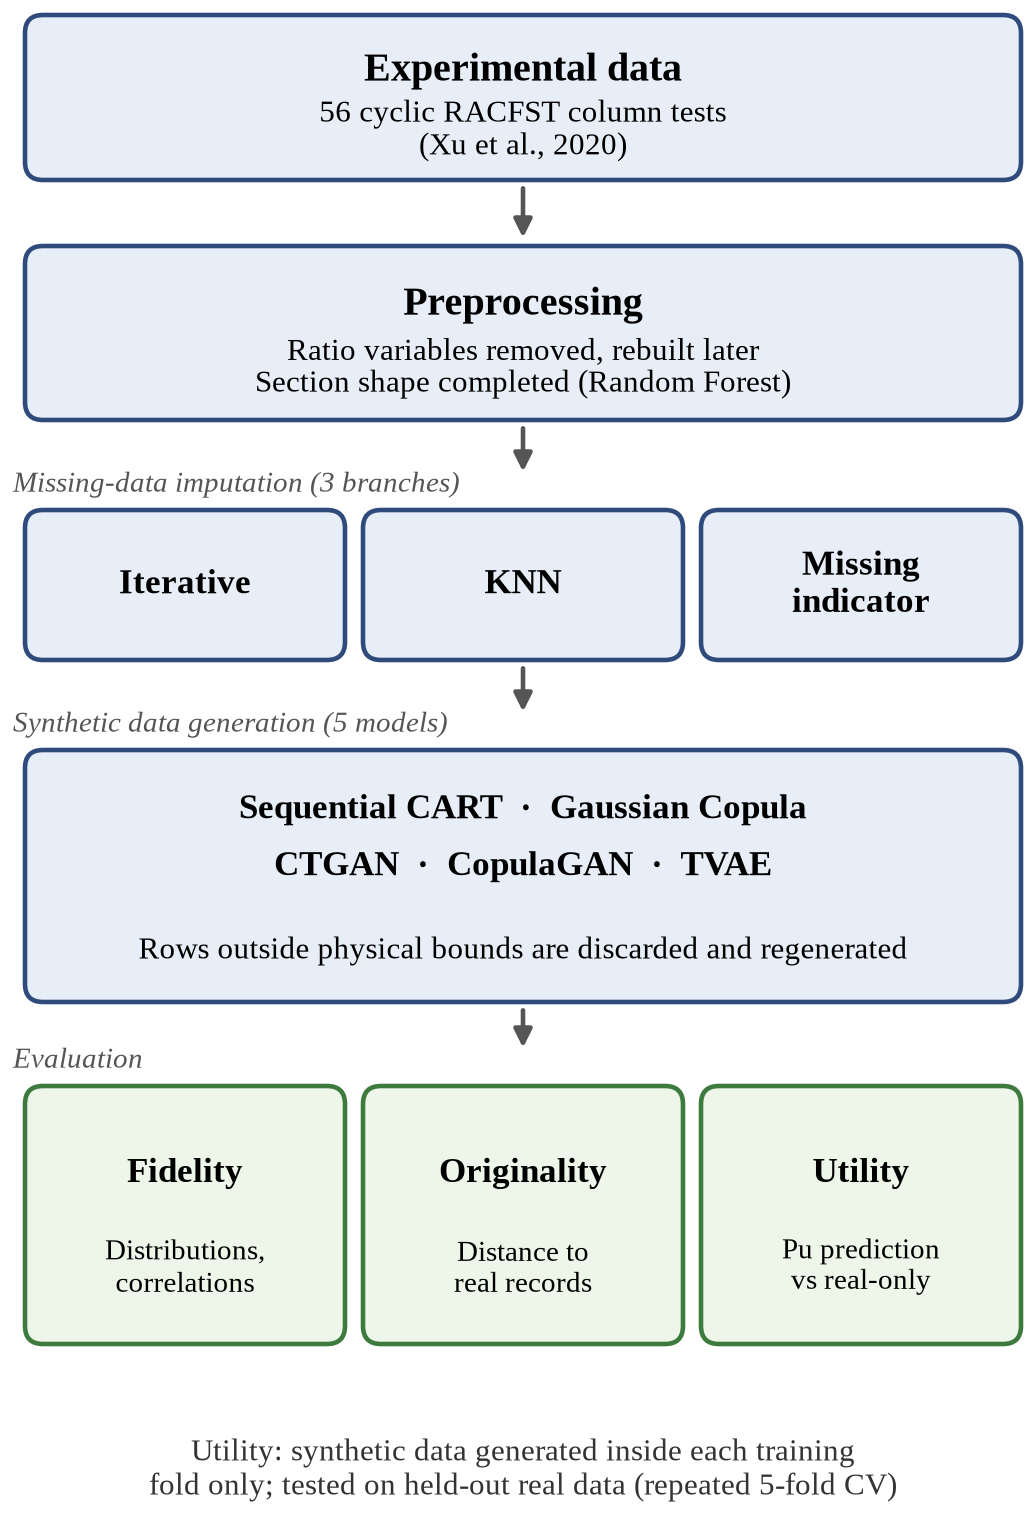
\includegraphics[width=0.55\textwidth]{figures/fig_flowchart.png}
\caption{Workflow of the RACFST benchmark. Imputation and generation are repeated inside every training fold for
the utility evaluation; the fidelity and originality evaluation uses synthetic sets generated from the full
imputed database}\label{fig:flow}
\end{figure}

\subsection{Missing data}
Missing categorical values are completed with a Random Forest classifier trained on the numerical inputs.
Missing numerical values are completed by one of three methods, each forming a separate analysis branch:
iterative multivariate imputation \citep{vanbuuren2011mice}, $k$-nearest-neighbour imputation with $k=5$
\citep{troyanskaya2001knn}, and a missing-indicator branch in which values are filled with the median and binary
indicator columns are added for the generators and removed before the predictive models are trained. In the
utility evaluation, all imputers are fitted on the training fold only and applied to the test fold.

\subsection{Generators}
Five generators were compared.
\emph{Sequential CART} synthesises one variable at a time; each variable is modelled by a classification or
regression tree on the variables already synthesised, and new values are drawn from the observed values in the
selected leaf \citep{reiter2005cart,nowok2016synthpop}. The implementation follows synthpop, with a minimum leaf
size of 5 and kernel smoothing of numerical values.
\emph{Gaussian Copula} models each marginal distribution separately and joins them with a Gaussian copula.
\emph{CTGAN} is a conditional generative adversarial network for mixed-type tabular data, \emph{TVAE} is a
variational autoencoder for the same data type, and \emph{CopulaGAN} applies CTGAN after a copula-based
transformation of the marginals \citep{xu2019ctgan}. The last four were run with the default settings of the
Synthetic Data Vault library, version 1.39 \citep{patki2016sdv}. No generator was tuned. Every call to a
generator received a different seed drawn from a single master random stream, so that repeated batches differ
and the whole study is reproducible.

\subsection{Constraint-checked sampling}
Each generator produces candidate rows in batches. A row is accepted only if every numerical value lies within
the minimum and maximum of that column in the data the generator was fitted on (the training fold in the utility
evaluation); rejected rows are discarded and generation continues until the required number of rows is reached.
The batch size adapts to the observed acceptance rate (500 to 24,000 rows per batch), with a limit on the total
number of generated rows. Batches are not filtered on any statistical fidelity score, so that the fidelity
metrics reported in Sect.~\ref{sec:fidelity} describe the raw output of each generator after physical filtering.
For RACFST, synthetic rows are allocated equally between the two section shapes, without duplicating any row,
and the generators themselves are fitted on the unbalanced data.

\subsection{Fidelity and originality}\label{sec:metrics}
For the fidelity evaluation, each generator produced 500 rows from the full imputed database in each imputation
branch. With the real data $X$ and synthetic data $Y$ restricted to numerical columns, the following quantities
were computed.
\begin{itemize}
\item \emph{Boundary score}: the fraction of synthetic values inside the real minimum--maximum range, averaged
over columns.
\item \emph{Correlation similarity}: $1 - \overline{|R_X - R_Y|}$, where $R$ is the Pearson correlation matrix and
the mean is over off-diagonal entries.
\item \emph{Covariance similarity}: $\max\left(0,\, 1 - \lVert C_X - C_Y \rVert_F / \lVert C_X \rVert_F\right)$,
where $C$ is the covariance matrix after standardising both data sets with the real means and standard
deviations.
\item \emph{Wasserstein distance} (WD): the one-dimensional Wasserstein distance between real and synthetic
values, averaged over columns.
\item \emph{Fr\'echet distance} (FD): $\lVert \mu_X - \mu_Y \rVert^2 + \mathrm{tr}\left(C_X + C_Y -
2(C_X C_Y)^{1/2}\right)$, computed on unstandardised values \citep{heusel2017fid}.
\item \emph{Distance to closest record} (DCR): the Euclidean distance, in standardised units, from each synthetic
row to its nearest real row; a value of zero indicates a copied record.
\item \emph{Propensity score}: $1 - 2|0.5 - \mathrm{AUC}|$, where AUC is the area under the ROC curve of a
shallow gradient-boosted classifier trained to distinguish real from synthetic rows
\citep{snoke2018utility}; 1 means the classifier cannot tell them apart and 0 means it separates them perfectly.
\end{itemize}
WD and FD are computed on unstandardised values and are therefore dominated by the columns with the largest
numerical range; they are reported for comparison between generators on the same database only.

\subsection{Predictive utility on the RACFST database (E0)}\label{sec:e0}
Utility was measured with repeated 5-fold cross-validation (3 repeats, 15 test folds). In each fold, imputation
was fitted on the training fold, each generator was fitted on the imputed training fold, and synthetic rows were
generated subject to the training-fold bounds; the derived ratios were then recomputed. Two predictive models were
trained for every fold, generator and imputation branch: one on the real training fold alone (real only) and one
on the real training fold plus the synthetic rows (augmented). Both were evaluated on the same real test fold. Two
augmentation ratios were tested: 1:1 (as many synthetic rows as real training rows) and a fixed 500 synthetic rows
per fold, which is about 11:1 for training folds of 44--45 tests.

The predictive models were Random Forest \citep{breiman2001rf} with 400 trees and XGBoost \citep{chen2016xgboost}
with 350 trees, maximum depth 4, learning rate 0.05 and row and column subsampling of 0.9. The settings were fixed
in advance and not tuned, because tuning within folds of 45 tests would itself be unstable. Performance is
reported as mean absolute error (MAE), root mean squared error and $R^2$ on the real test folds. The section shape
was also used as a classification target, but the real-only classifiers already reached a balanced accuracy of
1.0, so this task cannot show a benefit of augmentation and is not reported further.

\subsection{Training-size experiment (E1)}\label{sec:e1}
E1 asks whether 1:1 augmentation reduces prediction error when few real tests are available. Its design and
decision rule were committed to the public project repository before the experiment was run on any real data
(commit \texttt{0c3b2b0}, pushed 14 November 2026). For each of 20 draws, a random 25\% of the database was held
out as the test set and the remainder was shuffled; training sets were the first $n$ rows of the shuffled
remainder, with $n \in \{25, 50, 100, 200, 400\}$ for FRP-confined concrete and $n \in \{25, 50, 100, 150\}$ for
rectangular CFST, so that smaller training sets are nested in larger ones within a draw. In each training set,
iterative imputation was fitted on the training rows and applied to the test rows, each generator produced $n$
synthetic rows subject to the training-set bounds, and the two regressors were trained on the real rows alone and
on the real plus synthetic rows. The outcome for each draw is the relative change in test MAE,
\begin{equation}
d = \frac{\mathrm{MAE}_\mathrm{aug} - \mathrm{MAE}_\mathrm{real}}{\mathrm{MAE}_\mathrm{real}},
\end{equation}
so that negative values mean augmentation reduced error.

The registered decision rule was applied to every combination of database, training size, generator and
regressor (a \emph{cell}). A cell shows a \emph{Benefit} if the median of $d$ over the 20 draws is at most
$-0.05$ and a one-sided Wilcoxon signed-rank test \citep{wilcoxon1945} of $\mathrm{MAE}_\mathrm{aug} <
\mathrm{MAE}_\mathrm{real}$ gives $p < 0.05$ after Holm correction \citep{holm1979} over all cells of that
database (50 for FRP-confined concrete, 40 for rectangular CFST). \emph{Harm} is defined symmetrically. All other
cells show no detectable effect. The registered main claim, that augmentation helps in the small-data regime,
would be supported only if the same generator showed a Benefit at $n \leq 50$ on both databases for at least one
regressor.

Two deviations from the registered plan occurred and are reported here. First, the circular CFST subset (93
tests, $n \in \{25, 50\}$) was added after registration; it is analysed with the same rule but reported separately
and does not count towards the main claim. Second, the FRP run stopped at draw 14 because a confinement type
present in a test set was absent from the 25 training rows and the imputation code failed when decoding it. The
code was corrected to treat such values as missing, which changes only the case that had failed, and the run was
resumed from draw 14; draws 1--13 were unaffected.

\subsection{Software and reproducibility}
All analyses were run in Python 3.11 with scikit-learn \citep{pedregosa2011sklearn}, XGBoost, SciPy and the
Synthetic Data Vault. Exact package versions, the code, the derived database files and the registration record
are in the public repository (see Declarations).

%% ---------------------------------------------------------------------------------------------------------
\section{Results}\label{sec:results}

\subsection{Fidelity and originality on the RACFST database}\label{sec:fidelity}
Table~\ref{tab:fidelity} lists the fidelity and originality metrics. Every directly generated value lay within the
physical bounds; boundary scores below 1 (\boundMin--\boundMax) arise only from the recomputed ratios $w/c$,
$D/t$ and $L/D$, which combine bounded components but are not bounded themselves. The generators differed in how
well they preserved the joint structure of the data. Sequential CART had the highest covariance similarity under
\cartCovWins{} imputation branches (\cartCovMin--\cartCovMax), the lowest Fr\'echet distance under
\cartFdWins{} and the lowest Wasserstein distance under \cartWdWins. CTGAN and CopulaGAN retained little of the covariance structure (\ganCovMin--\ganCovMax). The
propensity score was at most \propMax{} for every generator, meaning that a simple classifier could distinguish
the synthetic rows of every generator from the real tests.

\begin{table}[t]
\caption{Fidelity and originality of 500 synthetic rows per generator, RACFST database. Bound.: boundary score;
Corr., Cov.: correlation and covariance similarity (higher is better); WD, FD: Wasserstein and Fr\'echet distance
(lower is better); DCR$_\text{mean}$: mean distance to the closest real record (standardised units); Prop.:
propensity score (1 = indistinguishable from real). Bold: best value within an imputation branch}\label{tab:fidelity}
\footnotesize
\input{generated/tab_fidelity.tex}
\end{table}

No synthetic row was a copy of a real test (minimum DCR \dcrMinAll{} across all generators and branches).
Sequential CART and TVAE produced rows closest to the real tests (mean DCR \dcrNearMin--\dcrNearMax), and the
copula and GAN generators produced rows farther away (\dcrFarMin--\dcrFarMax). Figure~\ref{fig:pca} shows the
synthetic rows in the first two principal components of the pooled real and synthetic data.

\begin{figure}[t]
\centering
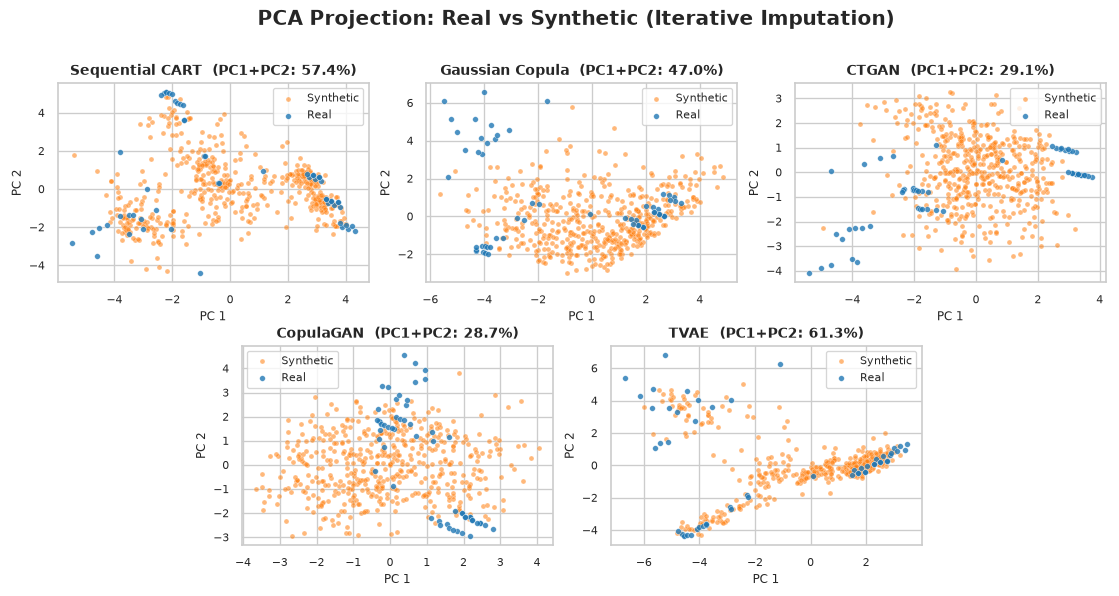
\includegraphics[width=\textwidth]{figures/fig_pca_iter.png}
\caption{Real tests and synthetic rows of each generator projected onto the first two principal components of
the pooled data (iterative imputation)}\label{fig:pca}
\end{figure}

\subsection{Predictive utility on the RACFST database}\label{sec:utility}
Table~\ref{tab:regression} gives the mean test MAE over the 15 folds. Models trained on the real data alone had
MAEs of \realMaeMin--\realMaeMax~kN ($R^2$ \realRtwoMin--\realRtwoMax). With 1:1 augmentation, the mean MAE was
lower than the real-only value in \regBetterOne{} of \regSettings{} generator, imputation and regressor settings
(all with \regBetterOneRegs, for \regBetterOneGens), by \regBetterOnePctMin\% to \regBetterOnePctMax\% (at most \regBestGainOne~kN). These
reductions were not consistent across folds: the augmented model had the lower error in only
\regBetterOneWinsMin{} to \regBetterOneWinsMax{} of the 15 folds, and no paired difference approached
significance (two-sided Wilcoxon signed-rank test, smallest uncorrected $p = \regBetterOnePMin$). In the other
\regWorseOne{} settings the mean MAE increased, by \regWorseOnePctMin\% to \regWorseOnePctMax\% (up to
\regWorseOneKnMax~kN). With 11:1 augmentation, the mean MAE was lower in \regBetterEleven{} of
\regSettings{} settings, and the increase ranged from \regElevenMin{} to \regElevenMax~kN.
Figure~\ref{fig:ratio} summarises the change in MAE by generator and ratio.

\begin{table}[t]
\caption{Mean test MAE (kN) over 15 cross-validation folds for $P_u$ of RACFST columns. RF: Random Forest; XGB:
XGBoost. Bold: lower than the real-only model in the same column}\label{tab:regression}
\footnotesize
\input{generated/tab_regression.tex}
\end{table}

\begin{figure}[t]
\centering
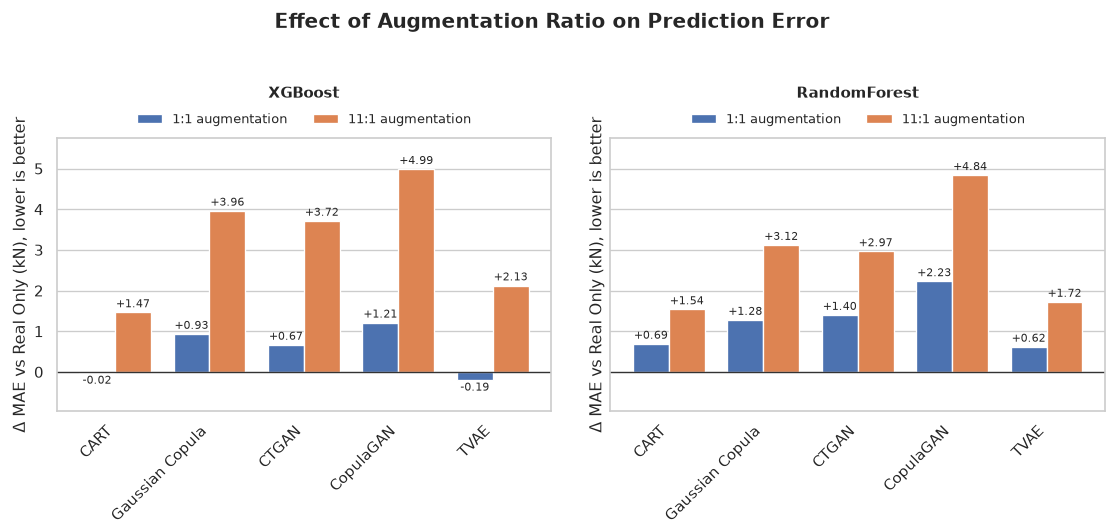
\includegraphics[width=\textwidth]{figures/fig_ratio.png}
\caption{Change in mean test MAE relative to the real-only model, averaged over the three imputation branches,
for 1:1 and 11:1 augmentation. Values above zero mean that augmentation increased the error}\label{fig:ratio}
\end{figure}

The largest single-fold error of the real-only Random Forest under iterative imputation was \worstRealRF~kN; with
1:1 sequential CART augmentation the largest single-fold error was \worstCartRF~kN (XGBoost: \worstRealXGB{} and
\worstCartXGB~kN). This difference concerns one fold out of fifteen and is not accompanied by a lower mean error,
so it is not evidence of a systematic benefit.

\subsection{Training-size experiment}\label{sec:e1res}
All generators produced the required rows in every draw (\eoneFailures{} generation failures). Real-only models
improved steadily with training size; for example, the median $R^2$ for FRP-confined concrete rose from
\rtwoFrpSmall--\rtwoFrpSmallHi{} at $n=25$ to \rtwoFrpLarge--\rtwoFrpLargeHi{} at $n=400$.

Figure~\ref{fig:e1} and Table~\ref{tab:e1} summarise the effect of augmentation. Of the \eoneCells{} registered
cells, \eoneBenefit{} showed a Benefit, \eoneHarm{} showed Harm and \eoneNone{} showed no detectable effect
(FRP-confined concrete: \eoneFrpHarm{} Harm, \eoneFrpNone{} no detectable effect; rectangular CFST:
\eoneRectHarm{} Harm, \eoneRectNone{} no detectable effect). The registered main claim is therefore not
supported. Harm became more frequent as the real training set grew: on FRP-confined concrete, sequential CART,
CTGAN, CopulaGAN and TVAE increased the error in \frpBigHarm{} of \frpBigCells{} cells with $n \geq 100$, with
median increases of \frpBigMin\% to \frpBigMax\%. Gaussian Copula was the only generator that rarely increased the
error (Harm in \gcHarm{} of \gcCells{} registered cells), but its median changes (\gcMin\% to \gcMax\%) did not
meet the Benefit criterion in any cell. The exploratory circular CFST subset showed the same pattern
(\eoneCircBenefit{} Benefit, \eoneCircHarm{} Harm, \eoneCircNone{} no detectable effect in \eoneCircCells{}
cells). The median change for every cell is listed in Appendix~\ref{app:cells}.

\begin{figure}[t]
\centering
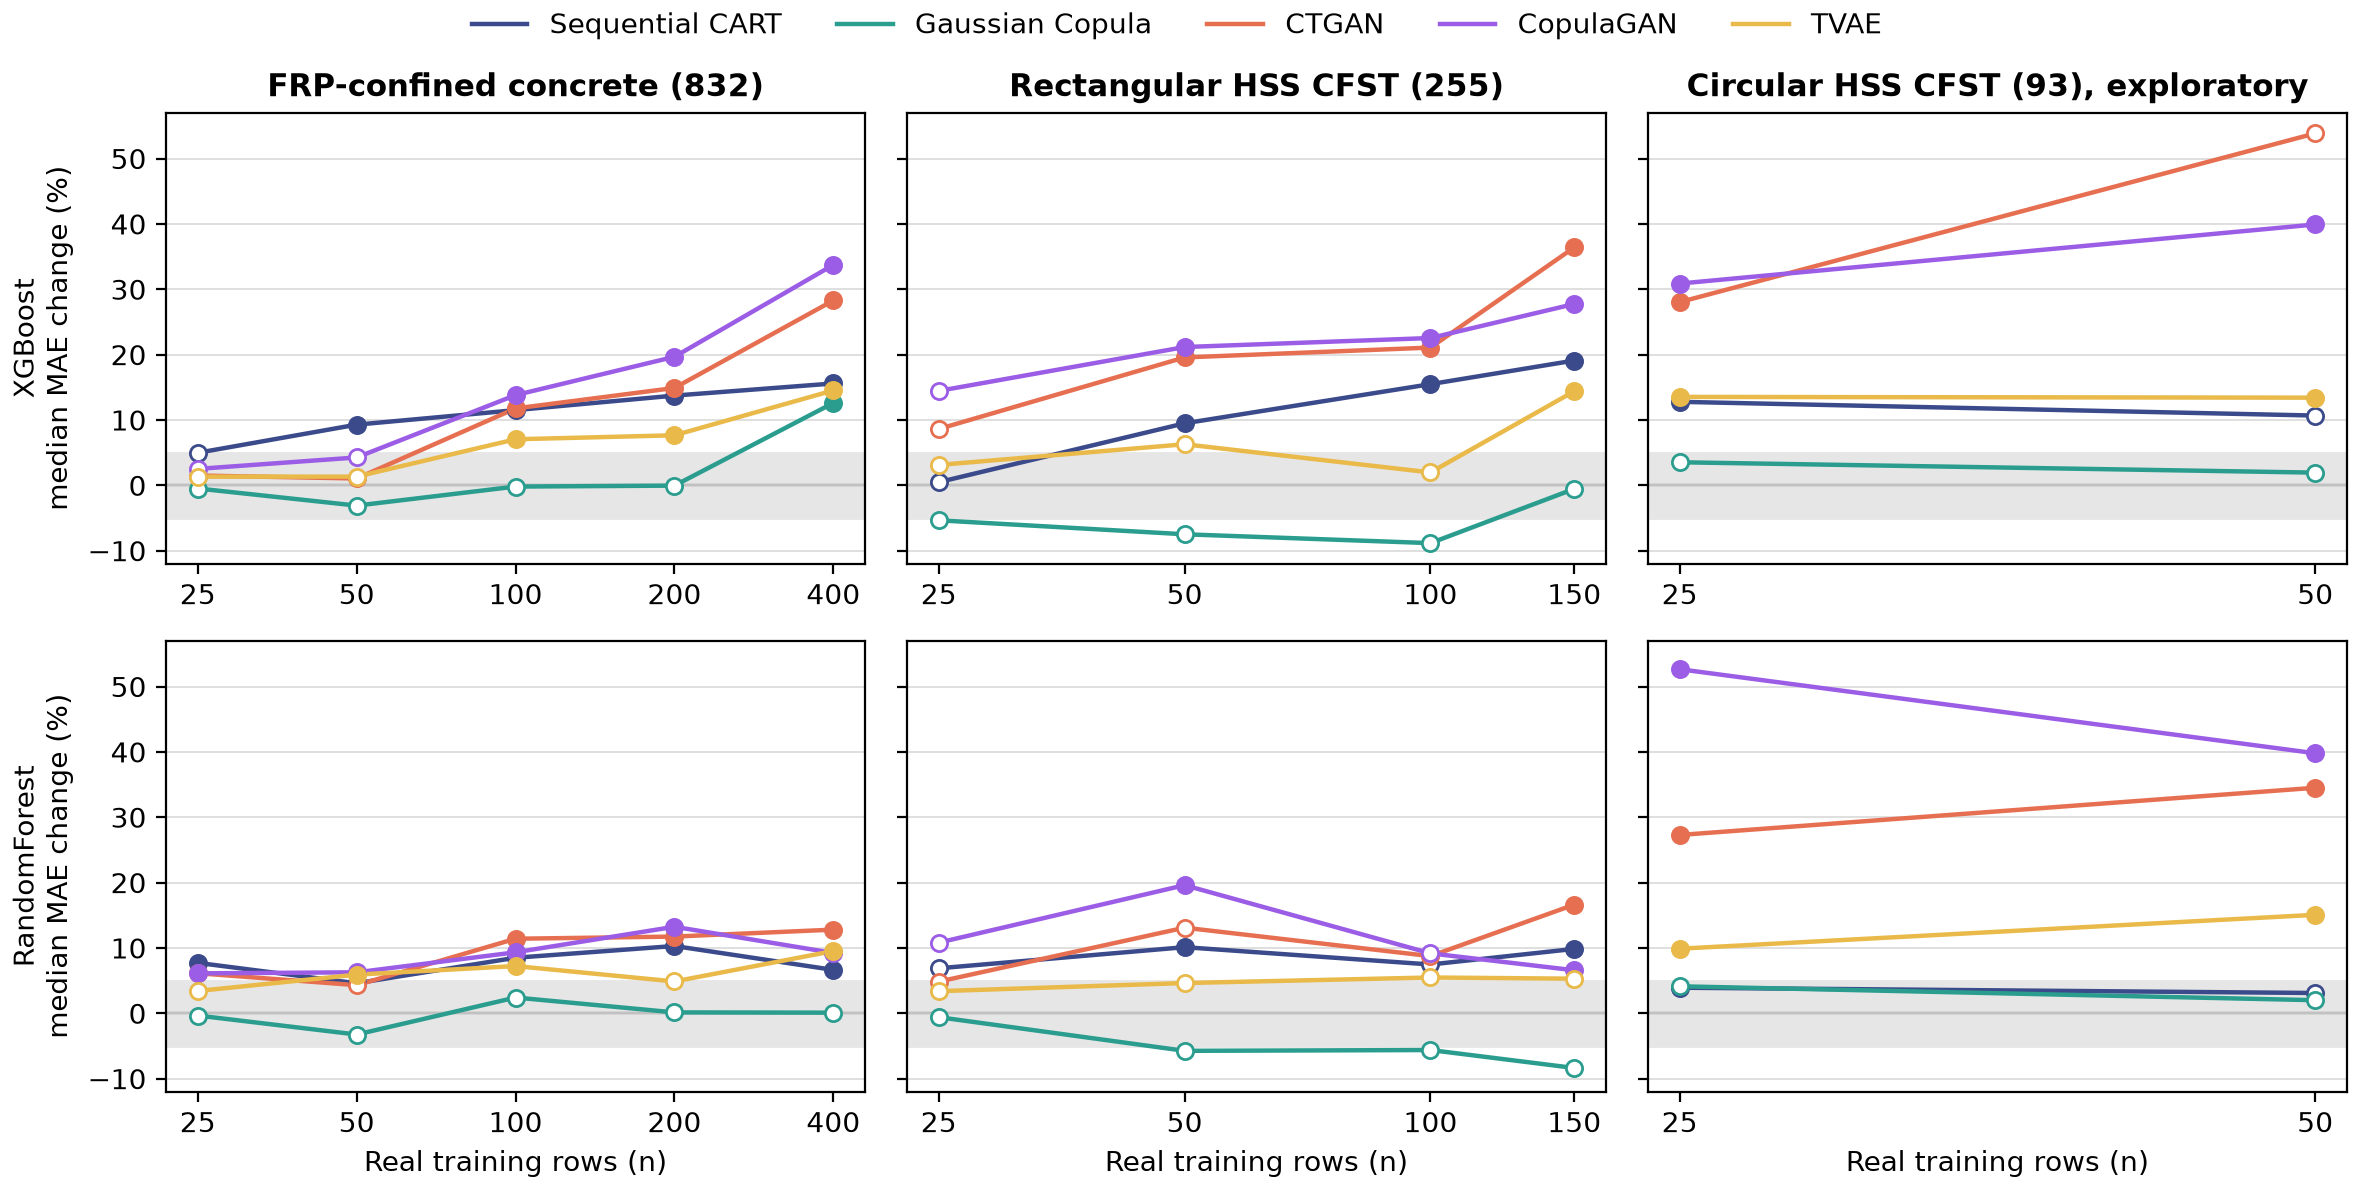
\includegraphics[width=\textwidth]{figures/fig_e1.png}
\caption{Median relative change in test MAE from 1:1 augmentation over 20 draws, by real training size. Filled
markers: cells with a Benefit or Harm verdict under the pre-registered rule; hollow markers: no detectable effect.
Grey band: $\pm5\%$. The circular CFST panel is exploratory}\label{fig:e1}
\end{figure}

\begin{table}[t]
\caption{Verdicts of the pre-registered rule per database and generator (cells = training sizes $\times$ two
regressors) and range of the median relative change in test MAE. $^{\dagger}$Exploratory}\label{tab:e1}
\footnotesize
\input{generated/tab_e1_counts.tex}
\end{table}

%% ---------------------------------------------------------------------------------------------------------
\section{Discussion}\label{sec:discussion}

\subsection{Fidelity does not imply utility}
Sequential CART reproduced the joint structure of the RACFST data better than the other generators, consistent
with its use in statistical disclosure control, where preserving relationships between variables is the main
requirement \citep{nowok2016synthpop}. Its synthetic rows nevertheless did not reduce prediction error consistently, and in the
training-size experiment they increased it as often as those of CopulaGAN and more often than those of the
other generators. A
plausible explanation is that synthetic rows drawn from trees fitted to the training data repeat the information
in the training data with added noise: a tree ensemble trained on the augmented set receives no new information
about the physical response and must fit the noise as well. This explanation was not tested directly in this
study. The deep generators preserved less of the structure of the data and harmed prediction most when the real
training set was largest, which is consistent with synthetic noise outweighing any regularising effect once the
real data alone support an accurate model.

\subsection{Relation to earlier reports of benefit}
\citet{song2024fire} reported that CTGAN with random oversampling improved the prediction of the fire resistance
of CFST columns. The present results do not contradict that finding for their database, but they show that a
benefit cannot be assumed for other structural databases, and they suggest that comparisons should include a
real-only model evaluated on the same test data, with imputation and generation confined to the training data.
Without these controls, part of an apparent benefit can arise from the evaluation design rather than from the
synthetic data.

\subsection{Practical recommendations}
For small structural databases, the results support three recommendations. First, a real-only baseline evaluated
on identical splits should accompany any augmented model. Second, if augmentation is used, the synthetic share
should be small, since the 11:1 ratio increased error for every generator. Third, fidelity scores should not be
used as a proxy for utility; a generator that preserves the covariance structure well can still degrade
predictions. In addition, where a database contains several specimens per test series, splits that hold out
whole series give a more realistic estimate of accuracy for new designs than random splits
(Sect.~\ref{sec:limits}).

\subsection{Limitations}\label{sec:limits}
The generators were used with library default settings; tuned generators, or more recent methods such as
CTAB-GAN \citep{zhao2021ctabgan} and diffusion models \citep{kotelnikov2023tabddpm}, may behave differently. The
training-size experiment used only the 1:1 ratio and the iterative imputation branch, and the regressors were not
tuned. The targets were used in their original units; capacities normalised by a plastic resistance, or
log-transformed, could change the relative behaviour of the real-only and augmented models. For FRP-confined
concrete, the inputs include the ultimate axial strain and the hoop rupture strain, which are measured at
failure; the task is therefore a consistency model for test data rather than a pre-test design prediction, and
both the real-only and augmented models used the same inputs. The FRP data were extracted from the published
tables and checked for internal consistency, but not compared value by value with the 99 original studies. The
RACFST tests come from \seriesCount{} test series (same section shape, outer dimension and wall thickness), and
specimens within a series differ mainly in axial load ratio and replacement ratio. Random cross-validation folds
therefore contain sister specimens of every test series, and the E0 results describe prediction within known
series. In a supplementary check with real data only and simple median imputation, the mean MAE was
\seriesMaeRandRF~kN (Random Forest) and \seriesMaeRandXGB~kN (XGBoost) with random folds, but
\seriesMaeLosoRF~kN and \seriesMaeLosoXGB~kN when each series was held out in turn ($R^2$ \seriesRtwoLosoRF{}
and \seriesRtwoLosoXGB), against a mean $P_u$ of \puMean~kN. Prediction for a new test series is therefore far less accurate than the random-fold results
suggest, and the effect of augmentation on that task was not examined. The larger databases in E1 also contain
several specimens per source study, so their random splits are likely to be optimistic to some degree. In
the RACFST table, the length and slenderness columns disagree for some studies; if the error lies in the length
column, the slenderness input is inconsistent between studies, which affects the real-only and augmented models
alike. The
maximum mean discrepancy was also computed but took the same value for every generator, because the kernel was
applied to unstandardised data, and it is not reported.

%% ---------------------------------------------------------------------------------------------------------
\section{Conclusions}\label{sec:conclusions}

Five tabular generators were benchmarked on a 56-test RACFST database with fold-local imputation and generation,
physical bounds on every synthetic row and a real-only baseline on identical folds, and a pre-registered
experiment tested augmentation at training sizes of 25 to 400 tests on two larger databases. The main findings
are as follows.
\begin{enumerate}
\item Sequential CART preserved the covariance structure of the RACFST data best; CTGAN and CopulaGAN preserved
little of it.
\item For the ultimate lateral load of RACFST columns, 1:1 augmentation lowered the mean error in
\regBetterOne{} of \regSettings{} settings, by at most \regBestGainOne~kN and not consistently across folds, and
raised it in the other \regWorseOne; 11:1 augmentation increased the error in every setting.
\item In the pre-registered experiment, augmentation showed no benefit in any of \eoneCells{} cells and a
statistically supported increase in error in \eoneHarm{}, more often at larger training sizes.
\end{enumerate}
Synthetic augmentation should therefore not be assumed to improve ML predictions for small structural test
databases, and claims of benefit should be supported by comparison with a real-only baseline on the same test
data.

%% ---------------------------------------------------------------------------------------------------------
\backmatter

\bmhead{Acknowledgements}
% AUTHORS: Springer Nature requires that use of large language models be documented (not as an author). Edit to
% match what was actually done before submission.
The authors used Claude (Anthropic), an AI assistant, for help with code development, analysis scripts and
drafting of the manuscript text. The authors checked the code, results and text and take full responsibility for
the content.

\section*{Declarations}

\begin{itemize}
\item \textbf{Funding} % AUTHORS: confirm
The authors did not receive support from any organisation for the submitted work.
\item \textbf{Competing interests} % AUTHORS: confirm
The authors have no competing interests to declare that are relevant to the content of this article.
\item \textbf{Ethics approval and consent to participate} Not applicable.
\item \textbf{Consent for publication} Not applicable.
\item \textbf{Data availability} The RACFST data are from \citet{xu2020racfst}. The FRP-confined concrete data
were extracted from \citet{ozbakkaloglu2013database}. The CFST data are from \citet{thai2021data} (CC BY 4.0).
The scripts that build the analysed files from these sources are available at
\url{https://github.com/dsquarre/SynthDataGen}.
\item \textbf{Code availability} The code, run outputs and the pre-registration record (commit \texttt{0c3b2b0})
are available at \url{https://github.com/dsquarre/SynthDataGen}.
\item \textbf{Author contribution} % AUTHORS: complete with each author's actual role (CRediT)
[To be completed by the authors.]
\end{itemize}

\begin{appendices}
\section{Median relative change in test MAE for every cell of the training-size experiment}\label{app:cells}

\begin{sidewaystable}
\caption{Median relative change in test MAE (\%) from 1:1 augmentation over 20 draws. Bold: Harm under the
pre-registered rule; no cell showed a Benefit. GC: Gaussian Copula. $^{\dagger}$Exploratory}\label{tab:cells}
\scriptsize
\input{generated/tab_e1_cells.tex}
\end{sidewaystable}
\end{appendices}

\bibliography{references}

\end{document}
